\subsection{Zustandshaltung der Pipeline}

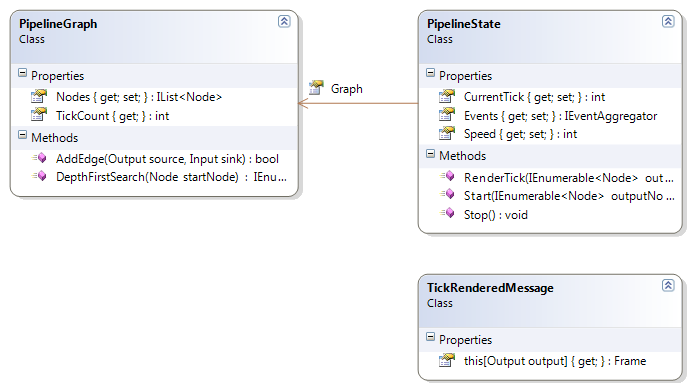
\includegraphics[width=\textwidth]{YuvKA.Pipeline/states.png}
Blablablubb PipelineState foo PipelineGraph bar.

\subsubsection{YuvKA.Pipeline.PipelineState}

\begin{verbatim}
[DataContract]
public class PipelineState
\end{verbatim}

\paragraph{Beschreibung}~\\
Die Klasse \name{PipelineState} vereint in sich den Gesamtzustand des Datenmodells, womit durch ihre Serialisierung alle relevanten Programmdaten gespeichert werden. Sie enthält den aktuellen Wiedergabestatus und bietet zur Wiedergabe eine Schnittstelle zum \name{PipelineDriver}.

\paragraph{Typmember}
\begin{itemize}

\property{FrameIndex}
	\begin{verbatim}
	[DataMember]
	public int FrameIndex { get; set; }
	\end{verbatim}
	Ruft den Index des zuletzt angezeigten Frames ab oder legt ihn fest. Das Neusetzen führt nicht zum erneuten Berechnen des Frames, sondern muss mit \name{Start} explizit angefordert werden.

\property{Speed}
	\begin{verbatim}
	[DataMember]
	public int Speed { get; set; }
	\end{verbatim}
	Ruft die Abspielgeschwindigkeit in Frames pro Sekunde ab oder legt sie fest.

\property{Graph}
	\begin{verbatim}
	[DataMember]
	public PipelineGraph Graph {get; set; }
	\end{verbatim}
	Ruft den \name{PipelineGraph} auf, der die Struktur der Pipeline repräsentiert und legt ihn fest.

\property{Events}
	\begin{verbatim}
	[Import(typeof(IEventAggregator))]
	public IEventAgggregator Events {get; set; }
	\end{verbatim}
	Per Dependency Injection injizierte Schnittstelle zum Caliburn Message System, über das die Ausgabefenster über die Beendigung der Berechnung eines Frames benachrichtigt werden.



\method{Start}
	\begin{verbatim}
	public void Start()
	\end{verbatim}
	Weist den \name{PipelineDriver} an, die Pipeline ab dem aktuellen \name{FrameIndex} zu berechnen.

\method{Stop}
	\begin{verbatim}
	public void Stop()
	\end{verbatim}
	Beendet die Wiedergabe und stoppt den \name{PipelineDriver}. Danach vom \name{PipelineDriver} asynchron erhaltene Frames werden ignoriert.
\end{itemize}

\subsubsection{YuvKA.Pipeline.PipelineGraph}
	
\begin{verbatim}
[DaraContract]
public class PipelineGraph	
\end{verbatim}

\paragraph{Beschreibung}~\\
Die Klasse \name{PipelineGraph} verwaltet den Aufbau des Pipeline-Graphen. 
	
\paragraph{Typmember}
\begin{itemize}

\property{Nodes}
	\begin{verbatim}
	[DataMember]
	public IList<Node> Nodes {get;}
	\end{verbatim}
	Verwaltet die im Pipeline-Graphen verfügbaren Knoten und gibt sie aus.

\property{FrameCount}
	\begin{verbatim}
	[DataMember]
	public int FrameCount {get;}
	\end{verbatim}
	Ruft die maximale Länge aller als Input gegebenen Videos auf.


	
\method{AddEdge}
	\begin{verbatim}
	public bool AddEdge(Output source, Input sink)
	\end{verbatim}
	Wenn die durch \name{source} und \name{sink} spezifizierte Kante zu keinem Zyklus innerhalb des Pipeline-Graphen führt, so soll sie durch setzen der Output-Property von \name{source} als \name{sink} hinzugefügt und true ausgegeben werden. Andernfalls soll die Kante nicht zum Graphen hinzugefügt und false ausgegeben werden.
\end{itemize}
	
\subsubsection{YuvKA.Pipeline.FrameRenderedMessage}
